\chapter{Fudamentação Teórica}
\label{fundamentacao}

{\color{red} Introdução...}

\section{Metodologias Ágeis}
\label{fundamentacao:ageis}

{\color{red} Metodologias Ágeis...}

\subsection{Fatores-Chave do Trabalho em Equipe}
\label{fundamentacao:ageis:fatores}

Como forma de elencar os fatores que influenciam o TE de equipes ágeis, foi realizada uma Revisão Literária, adotando características essenciais de Revisões Sistemáticas, para garantir uma maior quantidade de trabalhos relevantes encontrados. Apesar de não seguir o protocolo necessário para realizar uma Revisão Sistemática em Engenharia de \textit{Software} \cite{kitchenhan}, adotou-se nessa Revisão Literária duas etapas essenciais de Revisões Sistemáticas.

A primeira fase é de Seleção de Trabalhos, onde a relevância dos trabalhos para o contexto desta pesquisa foi avaliada com base nos títulos, \textit{abstracts} e palavras-chave desses trabalhos. Em seguida, com base nessas propriedades dos trabalhos, os estudos irrelevantes e duplicados são descartados. Depois disso, ocorre a fase de Extração dos Trabalhos, ou Avaliação da Qualidade dos Trabalhos. Nessa fase, os trabalhos considerados relevantes após a fase de Seleção de Trabalhos foram avaliados com base em suas introduções e conclusões, além de suas respectivas qualidades. Assim, são descartados mais alguns trabalhos. Finalmente, as informações relevantes para esta pesquisa foram extraídas dos trabalhos remanescentes.

Para realizar esse processo, os motores de busca selecionados para servir de fonte de trabalhos foram: \textit{ACM}\footnote{\url{http://dl.acm.org/}}, \textit{IEEE}\footnote{\url{http://ieeexplore.ieee.org/Xplore/home.jsp}}, \textit{Scopus}\footnote{\url{http://www.scopus.com/}}, \textit{Science Direct}\footnote{\url{http://www.sciencedirect.com/}} e \textit{Google Scholar}\footnote{\url{https://scholar.google.com.br/}}. Em seguida, foram definidas as \textit{strings} de busca para cada um desses motores. Além disso, foi utilizada a ferramenta \textit{StArt}\footnote{\url{http://lapes.dc.ufscar.br/tools/start_tool}} para auxiliar a gerência das informações referentes aos trabalhos encontrados.

Nesse processo de revisão de literária foram identificados 894 trabalhos. Ao final do processo, apenas 15 trabalhos foram considerados relevantes para o contexto da pesquisa. A Figura \ref{fundamentacao:ageis:fatores:revisao} contém informações mais detalhadas sobre os trabalhos relevantes selecionados ao longo do processo.

\begin{figure}[ht!]
\begin{center}
        \fbox{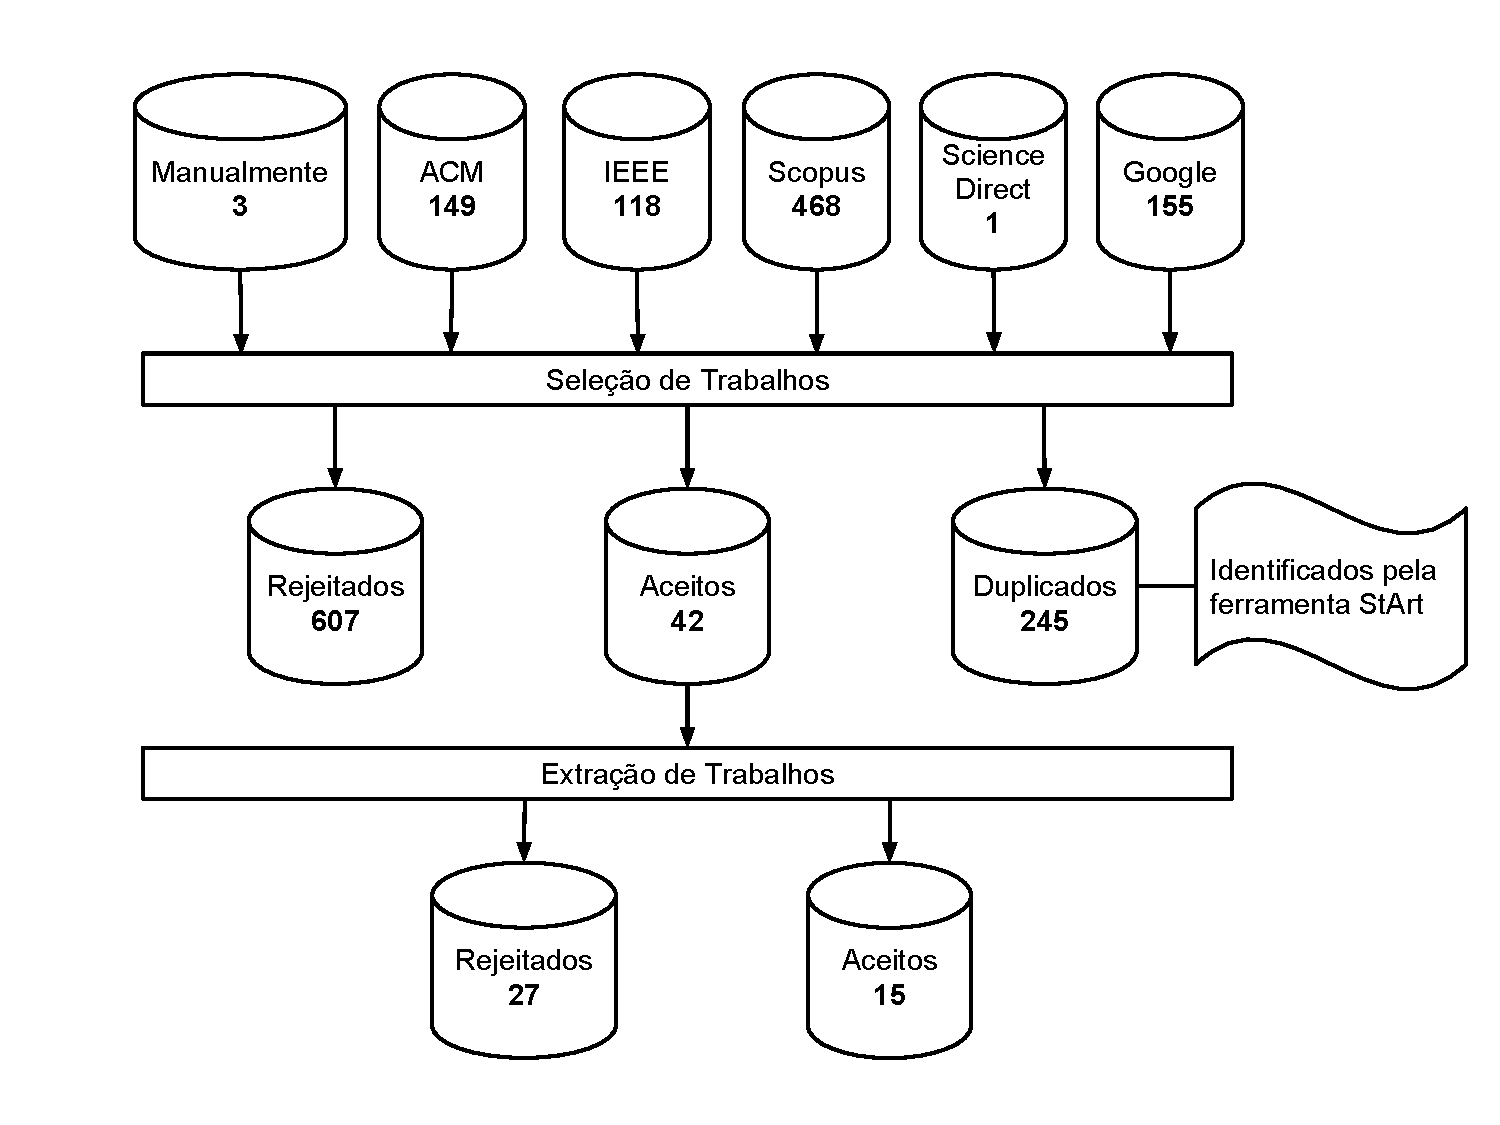
\includegraphics[scale=0.6]{figs/resultadosRevisao.pdf}}
    \end{center}
    \caption{Processo de seleção de trabalhos relevantes.}
    \label{fundamentacao:ageis:fatores:revisao}
\end{figure}

Finalmente, dentre os 15 trabalhos selecionados, foram identificados 20 fatores que influenciam a qualidade do TE em equipes ágeis. Esses fatores estão descritos na Tabela \ref{fundamentacao:ageis:fatores:tabela}.

\begin{table}[ht!]
\centering
\caption{Fatores-Chave que influenciam a qualidade do TE em projetos ágeis.}
\label{fundamentacao:ageis:fatores:tabela}
\resizebox{\textwidth}{!}{\begin{tabular}{|c|l|c|}
\hline
\textbf{Fator}                                                                            & \multicolumn{1}{c|}{\textbf{Conceito}}                                                                                                                                                                                                                                                         & \textbf{Referência} \\ \hline
Comunicação                                                                               & Compartilhamento de informações entre os membros da equipe.                                                                                                                                                                                                                                    &                     \\ \hline
Coordenação                                                                               & \begin{tabular}[c]{@{}l@{}}Refere-se à execução das atividades por parte dos integrantes da equipe\\ de maneira sincronizada e integrada.\end{tabular}                                                                                                                                         &                     \\ \hline
Coesão                                                                                    & \begin{tabular}[c]{@{}l@{}}Atração interpessoal dos membros da equipe, seu compromisso com as tarefas\\ da equipe, e espírito de grupo.\end{tabular}                                                                                                                                           &                     \\ \hline
Confiança                                                                                 & \begin{tabular}[c]{@{}l@{}}A vontade de uma das partes ser vulnerável às ações de outra parte com base\\ na expectativa de que o outro irá executar uma determinada ação importante \\ para o cedente, independentemente da capacidade de monitorar ou controlar\\ a outra parte.\end{tabular} &                     \\ \hline
\begin{tabular}[c]{@{}c@{}}Cooperação/\\ Colaboração/\\ Suporte Mútuo\end{tabular}        & Refere-se ao conceito de compromisso por parte do time como um todo.                                                                                                                                                                                                                           &                     \\ \hline
Diversidade de Valor                                                                      & Os membros da equipe compartilham dos mesmos valores e objetivos.                                                                                                                                                                                                                              &                     \\ \hline
Liderança Compartilhada                                                                   & Autoridade na tomada de decisões e liderança deve ser compartilhada.                                                                                                                                                                                                                           &                     \\ \hline
Orientação da Equipe                                                                      & Refere-se ao respeito mútuo entre os membros da equipe                                                                                                                                                                                                                                         &                     \\ \hline
Redundância                                                                               & \begin{tabular}[c]{@{}l@{}}Capacidade dos membros da equipe poderem substituir uns aos outros \\ na realização das atividades sem a necessidade de treinamento.\end{tabular}                                                                                                                   &                     \\ \hline
Autonomia da Equipe                                                                       & \begin{tabular}[c]{@{}l@{}}Refere-se à influência de agentes externos a equipe na realização das\\ atividades da equipe.\end{tabular}                                                                                                                                                          &                     \\ \hline
\begin{tabular}[c]{@{}c@{}}Aprendizagem da Equipe/\\ Adaptabilidade\end{tabular}          & \begin{tabular}[c]{@{}l@{}}Habilidade de identificar mudanças no ambiente da equipe e ajustar as\\ estratégias de acordo com o necessário.\end{tabular}                                                                                                                                        &                     \\ \hline
Monitoramento                                                                             & Sincronização da equipe com relação às atividades e problemas.                                                                                                                                                                                                                                 &                     \\ \hline
\textit{Feedback}                                                                         & \begin{tabular}[c]{@{}l@{}}Refere-se ao ato de prover, encaminhar e receber informações\\ relacionadas ao desempenho dos membros da equipe.\end{tabular}                                                                                                                                       &                     \\ \hline
Cultura                                                                                   & \begin{tabular}[c]{@{}l@{}}Conjunto de experiências, compreensões e significados compartilhados\\ entre os membros da equipe.\end{tabular}                                                                                                                                                     &                     \\ \hline
Personalidade                                                                             & Personalidade dos indivíduos que compõem a equipe.                                                                                                                                                                                                                                             &                     \\ \hline
Distribuição da Equipe                                                                    & A distribuição física da equipe.                                                                                                                                                                                                                                                               &                     \\ \hline
Tamanho da Equipe                                                                         & A quantidade de pessoas na equipe.                                                                                                                                                                                                                                                             &                     \\ \hline
\begin{tabular}[c]{@{}c@{}}Balanço das Contribuições\\ dos Membros da Equipe\end{tabular} & \begin{tabular}[c]{@{}l@{}}A capacidade de todos os membros da equipe contribuírem com todo\\ o conhecimento necessário para o desenvolvimento das atividades.\end{tabular}                                                                                                                    &                     \\ \hline
Esforço                                                                                   & \begin{tabular}[c]{@{}l@{}}Compartilhamento da carga de trabalho e priorização das tarefas da equipe\\ em relação a outras obrigações são indicadores do esforço de membros\\ da equipe para exercer as tarefas em comum.\end{tabular}                                                         &                     \\ \hline
Motivação                                                                                 & \begin{tabular}[c]{@{}l@{}}Motivação dos membros da equipe para realizar as atividades e trabalhar\\ em grupo.\end{tabular}                                                                                                                                                                    &                     \\ \hline
\end{tabular}}
\end{table}

A \textit{Comparative Agility}\footnote{\url{https://comparativeagility.com/}} é uma ferramenta web quer permite avaliar o quão ágil uma organização é em relação à outras. De acordo com o site, essa ferramenta é considerada a mais abrangente em relação à avaliação ágil na indústria. Essa avaliação é feita com base em um \textit{survey} organizado em sete dimensões e trinta e duas características. Uma das dimensões consideradas nessa ferramenta é o \textit{Trabalho em Equipe}. Essa dimensão é dividida em três características (i.e., Composição da Equipe, Gerenciamento e Comunicação). Para cada uma dessas características, há perguntas relacionadas a fatores que influenciam essas características. A Figura \ref{fundamentacao:ageis:fatores:comparativeagility} representa o relacionamento entre a dimensão \textit{Trabalho em Equipe}, suas características e os aspectos que contribuem para a boa qualidade dessas características.

\begin{figure}[ht!]
\begin{center}
        \fbox{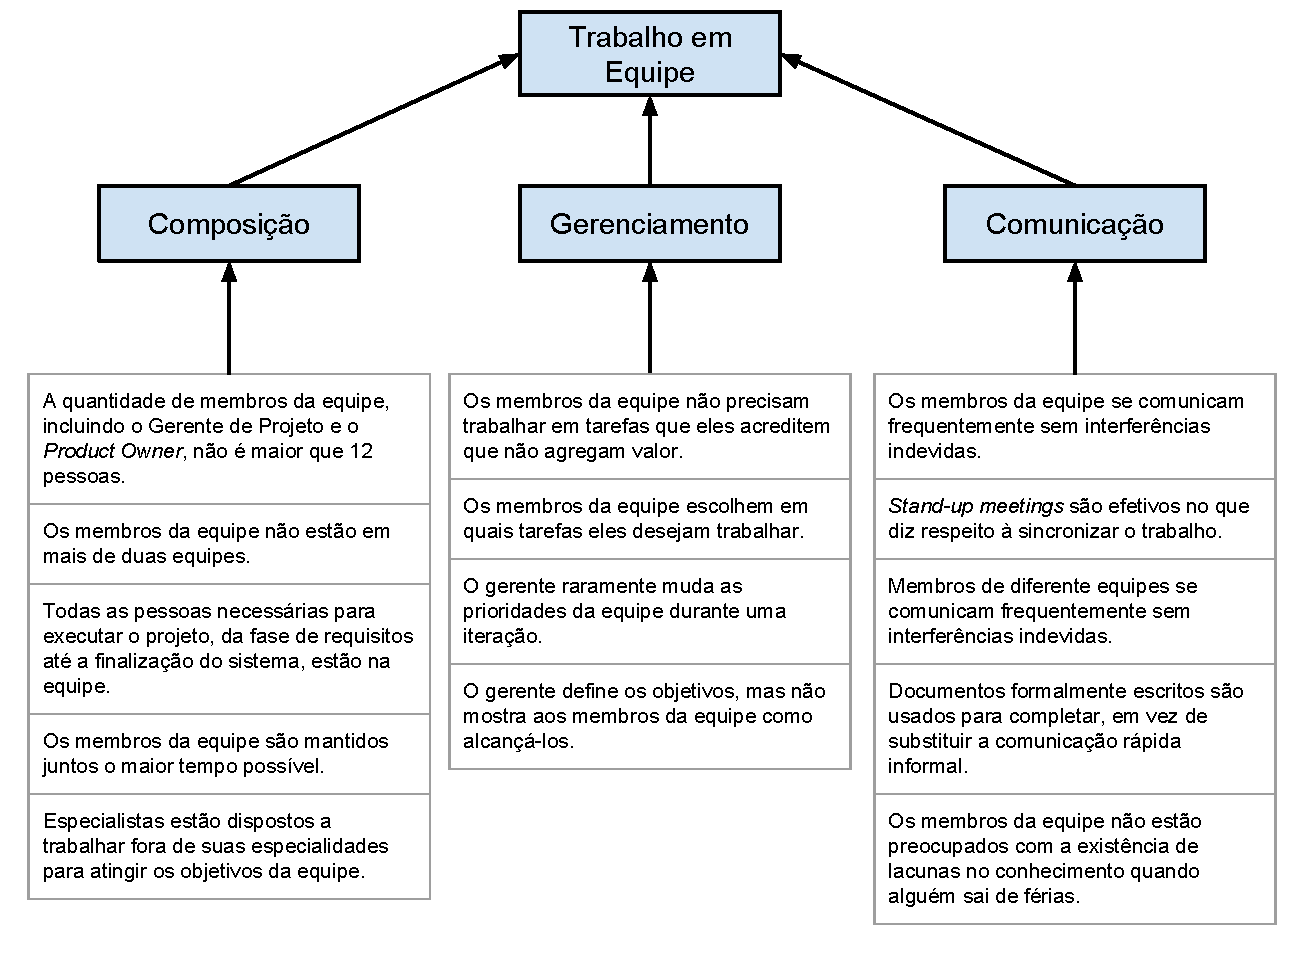
\includegraphics[scale=0.67]{figs/comparativeAgility_teamwork.pdf}}
    \end{center}
    \caption{Representação do Trabalho em Equipe na Ferramenta \textit{Comparative Agility}.}
    \label{fundamentacao:ageis:fatores:comparativeagility}
\end{figure}

\section{Redes Bayesianas}
\label{fundamentacao:redes}

{\color{red} Redes Bayesianas...}

\subsection{Construção de Redes Bayesianas}
\label{fundamentacao:redes:construcao}

{\color{red} Construção...}

\subsection{Nós Ranqueados}
\label{fundamentacao:nos}

{\color{red} Nós Ranqueados...}
